\documentclass[runningheads]{llncs}

% Submission is double-blind: \anonymoustrue hides the authors.
% Set \anonymousfalse for the camera-ready version.
\newif\ifanonymous
\anonymoustrue

% Shared preamble of main.tex and supplement.tex.
\usepackage[T1]{fontenc}
\usepackage{amsmath,amssymb}
\usepackage{stmaryrd}
\usepackage{graphicx}
\usepackage{booktabs}
\usepackage{tikz}
\usepackage{listingsutf8}
\usepackage{microtype}
\usepackage[hidelinks]{hyperref}
\pdfstringdefDisableCommands{\def\\{ }}

\lstdefinelanguage{Lean}{
  morekeywords={theorem,lemma,def,noncomputable,structure,instance,
                variable,import,namespace,end,open,scoped,where,
                fun,match,with,if,then,else,let,in,by,do,
                Prop,Type,Sort,deriving,inductive,abbrev,example,
                forall,exists,class,extends},
  sensitive=true,
  morecomment=[s]{/-}{-/},
  morecomment=[l]{--},
  literate=
    {->}{{$\rightarrow$}}{2}
    {→}{{$\rightarrow$}}{1}
    {↔}{{$\leftrightarrow$}}{1}
    {↦}{{$\mapsto$}}{1}
    {⟺}{{$\iff$}}{2}
    {∀}{{$\forall$}}{1}
    {∃}{{$\exists$}}{1}
    {∧}{{$\wedge$}}{1}
    {∨}{{$\vee$}}{1}
    {¬}{{$\neg$}}{1}
    {≤}{{$\le$}}{1}
    {≥}{{$\ge$}}{1}
    {≠}{{$\ne$}}{1}
    {∈}{{$\in$}}{1}
    {∉}{{$\notin$}}{1}
    {⊤}{{$\top$}}{1}
    {⊥}{{$\bot$}}{1}
    {⊔}{{$\sqcup$}}{1}
    {⊓}{{$\sqcap$}}{1}
    {⋁}{{$\bigvee$}}{1}
    {⨆}{{$\bigsqcup$}}{1}
    {∑}{{$\sum$}}{1}
    {∞}{{$\infty$}}{1}
    {ℝ}{{$\mathbb{R}$}}{1}
    {ℕ}{{$\mathbb{N}$}}{1}
    {ℤ}{{$\mathbb{Z}$}}{1}
    {Ω}{{$\Omega$}}{1}
    {δ}{{$\delta$}}{1}
    {μ}{{$\mu$}}{1}
    {ρ}{{$\rho$}}{1}
    {ι}{{$\iota$}}{1}
    {σ}{{$\sigma$}}{1}
    {ω}{{$\omega$}}{1}
    {∪}{{$\cup$}}{1}
    {∂}{{$\partial$}}{1}
    {×}{{$\times$}}{1}
    {⁻¹}{{${}^{-1}$}}{2}
    {ᶜ}{{${}^{\mathsf{c}}$}}{1}
    {ᶜᶜ}{{${}^{\mathsf{cc}}$}}{2}
    {⟨}{{$\langle$}}{1}
    {⟩}{{$\rangle$}}{1}
    {∘}{{$\circ$}}{1}
    {≡}{{$\equiv$}}{1}
    {∅}{{$\emptyset$}}{1}
    {▷}{{$\triangleright$}}{1}
    {⊆}{{$\subseteq$}}{1}
    {≃}{{$\simeq$}}{1}
    {Σ}{{$\Sigma$}}{1}
    {⋃}{{$\bigcup$}}{1}
    {⨅}{{$\bigsqcap$}}{1}
    {∣}{{$\mid$}}{1}
    {β}{{$\beta$}}{1}
    {κ}{{$\kappa$}}{1}
    {Θ}{{$\Theta$}}{1}
    {Γ}{{$\Gamma$}}{1}
    {Δ}{{$\Delta$}}{1}
    {α}{{$\alpha$}}{1}
    {₀}{{$_{0}$}}{1}
    {₁}{{$_{1}$}}{1}
    {₂}{{$_{2}$}}{1}
    {ˢ}{{$^{\mathsf{s}}$}}{1}
    {↑}{{$\uparrow$}}{1}
    {↓}{{$\downarrow$}}{1}
    {ψ}{{$\psi$}}{1}
    {φ}{{$\varphi$}}{1}
    {ν}{{$\nu$}}{1}
    {·}{{$\cdot$}}{1}
    {•}{{$\bullet$}}{1}
    {⊂}{{$\subset$}}{1}
    {∩}{{$\cap$}}{1}
    {⊕}{{$\oplus$}}{1}
    {⊗}{{$\otimes$}}{1}
    {⊸}{{$\multimap$}}{1}
    {ᵒᵖ}{{${}^{\mathsf{op}}$}}{2}
    {ᵇ}{{${}^{\mathsf{b}}$}}{1}
    {⥤}{{$\Rightarrow$}}{1}
}

\lstset{
  language=Lean,
  inputencoding=utf8/latin1,
  extendedchars=true,
  basicstyle=\ttfamily\small,
  keywordstyle=\bfseries,
  commentstyle=\itshape,
  showstringspaces=false,
  breaklines=true,
  xleftmargin=1em,
  aboveskip=0.6em,
  belowskip=0.6em,
}

\emergencystretch=3em
\interfootnotelinepenalty=10000

\newcommand{\ENNReal}{\ensuremath{[0,\infty]}}
\newcommand{\coh}{\mathrel{\asymp}}
\newcommand{\parr}{\mathbin{\rotatebox[origin=c]{180}{\&}}}
\newcommand{\Mix}{\mathrm{Mix}}
\newcommand{\STAB}{\mathrm{STAB}}
\newcommand{\QSTAB}{\mathrm{QSTAB}}
\newcommand{\loc}{\mathrm{loc}}
\newcounter{leanitem}
\renewcommand{\theleanitem}{L\arabic{leanitem}}
\newcommand{\leanitem}[1]{\par\noindent\refstepcounter{leanitem}\label{lean:#1}%
  \textsf{\textbf{\theleanitem}}\nopagebreak}
\makeatletter
\newcommand{\leanref}[1]{\textsuperscript{\textsf{\tiny\ref*{lean:#1}}}%
  \@ifnextchar\leanref{\textsuperscript{\textsf{\tiny,}}}{}}
\makeatother
\newcommand{\leanfootnotemark}{\textsuperscript{\textsf{\tiny$*$}}}
\newcommand{\leanfootnotetext}[1]{\begingroup
  \renewcommand{\thefootnote}{$*$}\footnotetext{#1}\endgroup}


\usepackage{xr}
\externaldocument{supplement}

\begin{document}

\title{Mixtures of Deterministic Programs in\\ Probabilistic Coherence Spaces}
\titlerunning{Mixtures of Deterministic Programs}

\ifanonymous
\author{Anonymous Author(s)}
\authorrunning{Anonymous}
\institute{Anonymous Institution}
\else
% TODO: Alex's surname, both affiliations, emails, ORCIDs.
\author{Polina Vinogradova\inst{1} \and Alex [SURNAME]\inst{2}}
\authorrunning{P. Vinogradova and A. [SURNAME]}
\institute{[AFFILIATION 1] \and [AFFILIATION 2]}
\fi

\maketitle

% !TEX root = main.tex
\begin{abstract}
Probabilistic coherence spaces (PCS) model higher-order probabilistic
programs.
We ask which elements of these spaces are mixtures of deterministic
programs, the results of choosing a deterministic program at random. For
each type of multiplicative--additive linear logic, we call the convex
hull of its deterministic elements its deterministic hull. Every PCS lies
between its deterministic hull and a local relaxation cut out
by the deterministic elements of the dual type. The orthogonal of the
deterministic hull of a type is the local relaxation of its dual. We
locate the PCS between these two bounds. At first order all
three sets coincide. At the type of a program that calls two functions,
the PCS is the whole local relaxation. When the data types
have at least two elements, it contains behaviours that no randomized
sequential program has, so some laws of sequential programs fail in the
model. At the dual type the PCS is the deterministic hull.
Its gap to the local relaxation is Bell's theorem. For duals of tensors of
additive types, induced four-cycles in the coherence graphs decide whether
a gap occurs. The gap then transfers to every formula over nonempty data
types in which such a tensor occurs negatively. The main results are
mechanized in Lean~4.

\keywords{Probabilistic coherence spaces \and Linear logic \and
Probabilistic programs \and Perfect graphs \and Contextuality \and Lean}
\end{abstract}


% !TEX root = main.tex
\section{Introduction}
\label{sec:intro}

A randomized program can be run by choosing a deterministic program at
random and running it. For first-order while programs, this gives the same
semantics as linear operators on measures~\cite{kozen1981}. We ask
whether it holds at higher types.

Probabilistic coherence spaces (PCS) are a model of linear logic in which a type
denotes a set of weight vectors on a set of points, its
web~\cite{girard2004,danos-ehrhard2011}. They are fully abstract for
probabilistic PCF, the extension of PCF (Programming Computable
Functions) with probabilistic
choice~\cite{ehrhard-pagani-tasson2018}. The proof of full abstraction
uses the form of the morphisms as power series, and not the definability
of every element of a space. In a concurrent game model of probabilistic
PCF, definability holds for the strategies that call one argument at a
time and depend only on the history they observe~\cite{castellan2018}.
We ask which elements of a space are mixtures of its elements with values in
$\{0,1\}$. Full abstraction does not settle this question, since it
concerns the equivalence of programs and not the laws valid on a whole
space. Such laws bound the behaviour of every program of a type at once. They
can fail on a space that contains more than the mixtures of deterministic
programs.

We call these elements the \emph{certain states} of a type. They are its
deterministic elements, and the set of their mixtures is their convex
hull, so we call it the \emph{deterministic hull} of the type. This is the construction of
generalized probabilism~\cite{paris2001,williams2012}, applied to the
points of a web. We work in multiplicative--additive linear logic (MALL)
over finite data types, whose programs use each argument exactly once. At
every MALL formula the deterministic hull lies inside the PCS. Each certain state is a clique of
Girard's coherence space. A
\emph{gap} is an element of the PCS outside the deterministic
hull. It violates a linear inequality that every certain state
satisfies~\cite{definetti1974,paris2001}.

The PCS also has an upper bound defined from certain states.
The \emph{local relaxation} of a formula is the set of weight vectors with
total weight at most $1$ on the support of every certain state of its
negation. It contains the PCS. Its orthogonal is the deterministic hull
of the negation. So every PCS lies between two sets defined from certain
states, and Table~\ref{tab:sandwich} shows where.

\begin{table}[t]
\centering
\caption{The PCS $P(A)$ between the deterministic hull and the
local relaxation of $A$. Strictness needs data types with at least two
elements, and in the last row it is shown over $\mathrm{Bool}$.}
\label{tab:sandwich}
\begin{tabular}{@{}llll@{}}
\toprule
$A$ & hull and $P(A)$ & $P(A)$ and relaxation & Sections \\
\midrule
$\mathbf{n} \multimap \mathbf{m}$ (first order) & equal & equal & \ref{sec:linear}, \ref{sec:duality-tight} \\
$T$ (second order) & strictly smaller & equal & \ref{sec:second}--\ref{sec:other}, \ref{sec:duality-local} \\
dual of $T$ & equal & strictly smaller & \ref{sec:exact-perfect}, \ref{sec:duality-bell} \\
$(T \otimes T)^{\perp}$ & strictly smaller & strictly smaller & \ref{sec:duality-shannon} \\
\bottomrule
\end{tabular}
\end{table}

At first order the three sets coincide: a probabilistic program from one
data type to another is a mixture of deterministic
programs~\cite{levin-peres-wilmer2009}. At the type
$T$ of a program that calls two functions once each, the deterministic
hull is the set of randomized sequential programs, by Kuhn's
theorem~\cite{kuhn1953}. It is the stable set polytope of a graph whose
clique-constrained polytope is the PCS. The PCS
is the whole local relaxation. When the data types have at least two
elements, the function with value $\tfrac12$ on five points of the web lies in the PCS and violates the
Klyachko--Can--Binicio\u{g}lu--Shumovsky (KCBS)
inequality~\cite{klyachko2008}, which every randomized sequential program
satisfies. So every law valid on the PCS of $T$ holds for
sequential programs, but not conversely.

At the dual of $T$, the tensor of the two argument types, the picture is
reversed. The PCS is the deterministic hull. When the data types have
at least two elements, it lies strictly inside the local relaxation. The Popescu--Rohrlich
box~\cite{popescu-rohrlich1994} lies in the local relaxation and outside
the PCS, so this gap is Bell's theorem. The two gaps are equivalent by the duality above. The deterministic hulls of a formula
and of its negation form a tight pair, each the orthogonal of the other,
iff neither has a gap. Tightness holds at first order and can fail at a tensor of first-order
types.

For the dual of a tensor of two formulas built from data types with
$\mathbin{\&}$ and $\oplus$, the gap is governed by induced four-cycles of
the coherence graphs. The direction without a gap has an explicit
decomposition, mechanized for formulas built from the unit type without
perfect graph theory. Coordinate retracts, embeddings of webs that
preserve the PCS in both directions, carry the gap to every
formula over nonempty data types in which such a tensor occurs
negatively. In quantum event logic no state has values in
$\{0,1\}$~\cite{kochen-specker1967}, so only the local relaxation
applies.

\paragraph{Contributions.}
\begin{enumerate}
  \item \textbf{Cliques.} Every certain state of a MALL formula is a clique
  of its coherence graph, but not conversely (Theorems~\ref{thm:mall}
  and~\ref{thm:shannon}).
  \item \textbf{Second order.} At $T$ the deterministic hull and the
  PCS are the stable set and the clique-constrained polytopes
  of one graph, with an explicit gap for two functional arguments
  (Theorems~\ref{thm:pentagon} and~\ref{thm:qstab}).
  \item \textbf{Exact condition.} For formulas built from data types with
  $\mathbin{\&}$ and $\oplus$, the dual of a tensor has no gap iff one
  factor has no induced four-cycle, with a direct proof mechanized over the
  unit type (Theorem~\ref{thm:second-exact}).
  \item \textbf{Transfer.} Coordinate retracts carry the gap to every
  formula over nonempty data types with such a tensor occurring negatively,
  a condition not necessary beyond second order (Theorem~\ref{thm:c4},
  Proposition~\ref{prop:f3}).
  \item \textbf{Duality.} Every PCS lies between the deterministic hull
  and the local relaxation, and the deterministic hulls of a formula and
  of its negation are tight iff neither has a gap, which holds at first
  order and can fail at a tensor of first-order types
  (Theorems~\ref{thm:loc-linear} and~\ref{thm:duality},
  Corollary~\ref{cor:tensor}).
\end{enumerate}

Every result of the paper is mechanized in Lean~4 over
\textsf{mathlib}~\cite{moura-ullrich2021,mathlib2020}, in about
$8{,}300$ lines, except steps the text marks as not formalized. A superscript number such as
\textsuperscript{\textsf{\scriptsize L1}} links a statement to its numbered
Lean counterpart. The archive in the data availability statement lists
the Lean statements.

% !TEX root = main.tex
\section{Mixtures of Certain States}
\label{sec:calculi}

This section describes a construction that takes a set of events and a
set of assignments that settle every event, and returns the set of
mixtures of these
assignments~\cite{definetti1974,paris2001,williams2012}. Later sections
apply it to the types of linear logic.
All functions take values in the
nonnegative reals $\mathbb{R}_{\ge 0}$.\footnote{The Lean development
works in the extended nonnegative reals $[0,\infty]$ of \textsf{mathlib},
the type in which measures take values. Every function in this paper takes
finite values, so the statements are the same, except that some Lean
statements carry a finiteness hypothesis that is automatic over
$\mathbb{R}_{\ge 0}$.}

\begin{definition}[presentation, deterministic hull\leanref{mix}]
\label{def:mix}
\begin{enumerate}
  \item[(i)] For a given set $E$, whose elements are the \emph{events},
  the \emph{certain states} of a \emph{presentation} $(E, S)$ are the
  elements of a set $S$ of functions $E \to \mathbb{R}_{\ge 0}$ with
  values in $\{0,1\}$. For $x : E \to \mathbb{R}_{\ge 0}$ and $e \in E$
  we write $x_e$ for $x(e)$, the weight that $x$ gives to $e$.
  \item[(ii)] For given functions $s_1, \dots, s_n : E \to \mathbb{R}_{\ge 0}$,
  the \emph{mixtures} of them are the functions $\sum_i w_i\, s_i$ such
  that $w_i \in \mathbb{R}_{\ge 0}$ and $\sum_i w_i = 1$.
  \item[(iii)] For a given presentation $(E, S)$, the \emph{deterministic hull}
  $\Mix(S)$ is the set of mixtures of certain states.
  \item[(iv)] For a given set $C$ of functions $E \to \mathbb{R}_{\ge 0}$,
  $C$ is \emph{closed under mixtures} if it contains every mixture of its
  elements.
\end{enumerate}
\end{definition}

\noindent
A certain state settles every event, with value $1$ or $0$, so the
certain states are the deterministic assignments and $\Mix(S)$ is their
convex hull, hence its name. A mixture
$\sum_i w_i s_i$ is the result of choosing a certain state at random,
$s_i$ with probability $w_i$: its value at an event $e$ is the
probability that the chosen state gives $e$ the value $1$. The deterministic hull
has an axiomatic description by linear inequalities.

\begin{definition}[affine law\leanref{affinelaw}]
\label{def:affine-law}
For a given finite set $E$, the \emph{affine laws} on $E$ are the
inequalities $\sum_{e \in E} a_e x_e + k \le \sum_{e \in E} b_e x_e + k'$
such that $a, b : E \to \mathbb{R}_{\ge 0}$ and
$k, k' \in \mathbb{R}_{\ge 0}$. The functions that \emph{satisfy} a law are
the $x : E \to \mathbb{R}_{\ge 0}$ such that the inequality is true at
$x$, and a law is \emph{valid on} a set of functions if every function in
the set satisfies it.
\end{definition}

\noindent
For finite $E$, $\Mix(S)$ is the set of
functions that satisfy every affine law valid on $S$, by the completeness
theorem of generalized probabilism~\cite{definetti1974,paris2001}\leanref{affinelaw-holds-of-mix}\leanref{mix-eq-laws}.
We call the affine laws valid on $S$ the \emph{laws of the presentation}.
The presentation is \emph{sound} for a set $C$ of functions if every law
of the presentation is valid on $C$.

\begin{definition}[gap]
\label{def:gap}
For a given presentation $(E, S)$, the sets with a \emph{gap} over $S$
are the sets $C$ of functions $E \to \mathbb{R}_{\ge 0}$ such that $C$
contains $S$, is closed under mixtures, and is not $\Mix(S)$.
\end{definition}

\noindent
A set that contains $S$ and is closed under mixtures contains $\Mix(S)$,
so a gap is a strict inclusion. An element of a gap does not arise from
choosing a certain state at random. The completeness theorem allows us to
characterize gaps by laws.

\begin{corollary}[a gap is a violated law\leanref{mix-eq-laws}]
\label{cor:gap-law}
Let $E$ be finite, and let $C$ be a set of functions
$E \to \mathbb{R}_{\ge 0}$ that contains $S$ and is closed under mixtures.
Then $C$ has a gap over $S$ iff some element of $C$ violates a law of the presentation, that is,
iff the presentation is not sound for $C$.
\end{corollary}

\noindent
A simple form of law bounds how
many events of a finite set $F \subseteq E$ a certain state can give the
value $1$. If no certain state gives the value $1$ to more than $k$
events of $F$, then $\sum_{e \in F} x_e \le k$ is a law of the
presentation, a \emph{counting law}. Many Bell and noncontextuality
inequalities, such as the Clauser--Horne--Shimony--Holt (CHSH) and the KCBS
inequalities, have this
form~\cite{pitowsky1991,cabello2014}, and every gap
found in this paper violates a counting law.


% !TEX root = main.tex
\section{Linear Logic}
\label{sec:linear}

In probabilistic coherence spaces a formula denotes a set of weight
vectors on a set of points~\cite{danos-ehrhard2011}. The construction of
Section~\ref{sec:calculi} applies to them, with the points as events and
the elements with values in $\{0,1\}$ as certain states.

\subsection{Coherence Spaces, Data Types, First Order}
\label{sec:linear-first}

\begin{definition}[probabilistic coherence space\leanref{ispcs-lin}]
\label{def:pcs}
\begin{enumerate}
  \item[(i)] For a given finite set $W$, the \emph{web}, whose elements are the
\emph{points}, the \emph{weight vectors} on $W$ are the functions
  $W \to \mathbb{R}_{\ge 0}$, and their pairing is
  $\langle x, y \rangle = \sum_{w \in W} x_w y_w$.
  \item[(ii)] For a given set $Q$ of weight vectors, the \emph{orthogonal}
  $Q^{\perp}$ is the set of weight vectors $y$ such that
  $\langle x, y \rangle \le 1$ for every $x \in Q$, and $Q^{\perp\perp}$
  is the \emph{biorthogonal} of $Q$.
  \item[(iii)] For a given web $W$, the \emph{probabilistic coherence
  spaces} (PCS) with web $W$ are the sets $P$ of weight vectors on $W$
  such that $P = P^{\perp\perp}$, every point $w$ has some $x \in P$ with
  $x_w \ne 0$, and for every point $w$ the values $x_w$ with $x \in P$
  are bounded~\cite{danos-ehrhard2011}.
\end{enumerate}
\end{definition}

\noindent
Every orthogonal is closed under mixtures, since
$\langle x, \sum_i w_i y_i \rangle = \sum_i w_i \langle x, y_i \rangle \le
\sum_i w_i = 1$\leanref{mix-subset-orth}. A PCS is the orthogonal of
$P^{\perp}$, so it is closed under mixtures.

For a finite set $X$, the \emph{data type} $X$ is the PCS of the
$x : X \to \mathbb{R}_{\ge 0}$ with $\sum_{a \in X} x_a \le 1$, the
subprobability distributions on $X$\leanref{ispcs-lin}. An element is
the output distribution of a computation with values in $X$, and
$1 - \sum_a x_a$ is the probability that it does not terminate. We write
$\mathbf{n}$ for the data type $\{1, \dots, n\}$, and $\mathrm{Bool}$ for
$\mathbf{2}$ with values $t$ and $f$. For data types $X$ and $Y$, the PCS
$X \multimap Y$ on the web $X \times Y$ is the set of
$t : X \times Y \to \mathbb{R}_{\ge 0}$ with
$\sum_{b} \sum_{a} x_a\, t(a,b) \le 1$ for every $x$ in $X$, equivalently
$\sum_{b} t(a,b) \le 1$ for every $a \in X$\leanref{mem-lin-iff}. These
are the substochastic matrices, the probabilistic programs from $X$ to
$Y$ that may not terminate, with $t(a,b)$ the probability of output $b$
on input $a$.

A \emph{coherence space} in the sense of Girard is a set with a reflexive
and symmetric relation, its \emph{coherence}~\cite{girard1987}. A
\emph{clique} is a set of pairwise coherent elements. In
$X \multimap Y$, two points $(a, b)$ and $(a', b')$ cohere iff they are
equal or $a \ne a'$. So the cliques are the graphs of partial functions
from $X$ to $Y$.

The implications $X \multimap Y$ between data types are the
\emph{first-order} types. Take as certain states the elements of
$X \multimap Y$ with values in $\{0,1\}$. Write $Y_{\bot}$ for $Y$ with
an added value $\bot$ for non-termination. For $f : X \to Y_{\bot}$, let $\det f(a, b) = 1$ if $f(a) = b$ and $0$ otherwise. We show that the
certain states are these deterministic programs and that
$X \multimap Y$ has no gap over them. Part (i) is known for stochastic
matrices~\cite[Prop.~1.5]{levin-peres-wilmer2009}, and we formalize it
for substochastic ones.

\begin{proposition}[first order~\cite{levin-peres-wilmer2009}\leanref{pcs-recipe}\leanref{sharp-lin-iff-clique}]
\label{prop:first-order}
Let $X$ and $Y$ be finite.
(i) $X \multimap Y = \Mix\{\det f \mid f : X \to Y_{\bot}\}$.
(ii) A function $t : X \times Y \to \mathbb{R}_{\ge 0}$ with values in
$\{0,1\}$ lies in $X \multimap Y$ iff its support is a clique of
$X \multimap Y$.
\end{proposition}

\noindent
For (i), each row $t(a, \cdot)$ is a
subprobability distribution on $Y$, and so a mixture of the point masses
and the zero vector. Choosing one of these independently for each row,
with the product of the weights, allows for expressing 
$t$ as a mixture of deterministic
programs. For (ii), a substochastic matrix with values in $\{0,1\}$ has
at most one entry $1$ in each row.

\subsection{MALL Formulas and Their Semantics}
\label{sec:linear-mall}

Multiplicative--additive linear logic (MALL) builds formulas from data
types with linear negation and two conjunctions~\cite{girard1987}. The
formula $A \otimes B$ is the type of a pair of independent elements of $A$
and of $B$. The formula $A \mathbin{\&} B$ is the type of an element that can be used
as an element of $A$ or of $B$.

\begin{definition}[formulas and their semantics\leanref{linear-fm}]
\label{def:mall}
\begin{enumerate}
  \item[(i)] The \emph{formulas} are the terms generated from the data
  types $\mathbf{n}$, for $n \in \mathbb{N}$, by linear negation
  $A^{\perp}$, the tensor $A \otimes B$, and the product
  $A \mathbin{\&} B$. The derived connectives are
  $A \parr B = (A^{\perp} \otimes B^{\perp})^{\perp}$,
  $A \oplus B = (A^{\perp} \mathbin{\&} B^{\perp})^{\perp}$, and
  $A \multimap B = (A \otimes B^{\perp})^{\perp}$.
  \item[(ii)] For a given formula $A$, the \emph{web} $|A|$ is
  $\{1, \dots, n\}$ for $\mathbf{n}$, $|A|$ for $A^{\perp}$,
  $|A| \times |B|$ for $A \otimes B$, and the disjoint union
  $|A| \sqcup |B|$ for $A \mathbin{\&} B$.
  \item[(iii)] For a given formula $A$, the PCS $P(A)$ is the data type
  $\mathbf{n}$ for $\mathbf{n}$, $P(A)^{\perp}$ for $A^{\perp}$,
  $\{ x \otimes y \mid x \in P(A),\ y \in P(B) \}^{\perp\perp}$ for
  $A \otimes B$, where $(x \otimes y)(a, b) = x_a y_b$, and the set of
  $z$ whose restrictions to $|A|$ and $|B|$ lie in $P(A)$ and $P(B)$ for
  $A \mathbin{\&} B$~\cite{danos-ehrhard2011}.
  \item[(iv)] For a given formula $A$, the \emph{coherence} $\coh_A$ is
  the relation on $|A|$ such that $s \coh_{\mathbf{n}} t$ iff $s = t$,
  $s \coh_{A^{\perp}} t$ iff $s = t$ or not $s \coh_A t$, two pairs cohere
  in $A \otimes B$ iff their first components cohere and their second
  components cohere, and points of $A \mathbin{\&} B$ cohere iff they
  cohere in $A$ or in $B$, or lie in different parts~\cite{girard1987}.
  The \emph{coherence graph} $G_A$ is the graph on $|A|$ whose edges are
  the pairs of distinct coherent points.
\end{enumerate}
\end{definition}

\noindent
The semantics computes the spaces of Section~\ref{sec:linear-first}:
$P(\mathbf{n} \multimap \mathbf{m})$ is the PCS
$\{1, \dots, n\} \multimap \{1, \dots, m\}$\leanref{p-lolli-base}, with
the coherence described there. So Proposition~\ref{prop:first-order} is
a statement about the formulas
$\mathbf{n} \multimap \mathbf{m}$\leanref{recipe-formula}.

The \emph{presentation} of a formula $A$ is $(|A|, S_A)$, where $S_A$ is
the set of elements of $P(A)$ with values in $\{0,1\}$, the
\emph{certain states} of $A$. The \emph{deterministic hull} of $A$ is
$\Mix(S_A)$.
Every $P(A)$ is a PCS~\cite{danos-ehrhard2011}\leanref{ispcs-p}, so it
contains the deterministic hull of $A$\leanref{recipe-subset-p}. Definition~\ref{def:gap}
therefore applies to it. We say that $A$ has a \emph{gap}
if $P(A)$ has a gap over the certain states of $A$, that is, if the
presentation of $A$ is not sound for $P(A)$ (Corollary~\ref{cor:gap-law}).

\subsection{Coherence at Every Formula}
\label{sec:linear-coherence}

We prove that the coherence bounds the weights of pairs of points,
and so constrains the certain states.

\begin{theorem}[coherence at every formula\leanref{linear-invariants}\leanref{sharp-isclique}]
\label{thm:mall}
Let $A$ be a formula. The indicator of every point and of every pair of
distinct coherent points lies in $P(A)$. Every $x \in P(A)$ satisfies
$x_s \le 1$ for every point $s$, and $x_s + x_t \le 1$ for every pair of
distinct incoherent points $s, t$. In particular, every certain state of
$A$ is the indicator of a clique of the coherence graph $G_A$.
\end{theorem}

\noindent
The proof is a simultaneous induction on $A$. Negation exchanges the
statement about coherent pairs with the statement about incoherent pairs.
For $A \otimes B$, the indicator of a coherent pair is bounded by the
tensor of the indicators of its two projections. A pair incoherent in
$A \otimes B$ is incoherent in one component, where the bound of $A$ or of
$B$ applies together with the bound on single points. So the bound on
incoherent pairs, the motivating intuition for probabilistic coherence
spaces~\cite{girard2004}, holds at every multiplicative--additive formula
over data types.


% !TEX root = main.tex
\section{Second Order}
\label{sec:second}

At first order there is no gap (Proposition~\ref{prop:first-order}). This
section shows that there is one at the second-order type of a program with
two functional arguments, and describes the deterministic hull there.

\subsection{Sequential Programs and Kuhn's Theorem}
\label{sec:second-seq}

Let $X, Y, X', Y'$ be data types. The formula
$K = (X \multimap Y) \otimes (X' \multimap Y')$ is the \emph{core}. Its negation $T = K^{\perp}$ is the type of a program that receives two programs
$f : X \multimap Y$ and $g : X' \multimap Y'$, calls each once, and then
terminates or does not. Its web is $(X \times Y) \times (X' \times Y')$. A point $((a, b), (c, d))$ records that the program called $f$ on
$a$ and received $b$, and called $g$ on $c$ and received $d$. By
Definition~\ref{def:mall}(iii), $P(T)$ is the orthogonal of the products: it
is the set of $t$ with $\sum_{p, q} y_p\, t(p, q)\, z_q \le 1$ for all
$y \in P(X \multimap Y)$ and $z \in P(X' \multimap Y')$\leanref{p-second}. For
arguments $y$ and $z$, the sum $\sum_{p,q} y_p\, t(p,q)\, z_q$ is the
probability that $t$ terminates.

A \emph{randomized sequential program} of type $T$ calls one argument
first. If it calls $f$ first, it chooses the input $a$ with probability
$\mu(a)$, after the answer $b$ chooses the input $c$ to $g$ with
probability $\kappa(a, b, c)$, and after the answer $d$ terminates with
probability $\rho(a, b, c, d)$. Its value at $((a, b), (c, d))$ is
$\mu(a)\, \kappa(a, b, c)\, \rho(a, b, c, d)$ plus the analogous term for
the branch that calls $g$ first, with $\sum \mu \le 1$ over both branches,
$\sum_c \kappa(a, b, c) \le 1$, and $\rho \le 1$. It is
\emph{deterministic} if its values are in $\{0,1\}$. We prove the
following, whose part (ii) is an instance of Kuhn's
theorem~\cite{kuhn1953}.

\begin{theorem}[second order\leanref{sharp-td-iff}\leanref{sharp-mem-sequentialg}\leanref{recipe-eq-sequentialg}]
\label{thm:second-order}
Let $X$ and $X'$ be nonempty.
(i) A function with values in $\{0,1\}$ lies in $P(T)$ iff its support
lies in a set $\{((a, b), (c(b), d)) \mid b \in Y,\ d \in Y'\}$ for some
$a \in X$ and $c : Y \to X'$, or in a set
$\{((a(d), b), (c, d)) \mid b \in Y,\ d \in Y'\}$ for some $c \in X'$ and
$a : Y' \to X$. These are exactly the deterministic sequential programs.
(ii) The deterministic hull of $T$ is the set of randomized sequential programs.
\end{theorem}

\noindent
The two sets in (i) are the decision trees of a program that calls $f$
first and of one that calls $g$ first. Part (ii) has two directions. Every randomized
sequential program is a mixture of deterministic
ones\leanref{sequentialg-subset-mix}. Every mixture of randomized
sequential programs is a randomized sequential
program\leanref{mix-sequentialg}.

For nonempty $X$ and $X'$, we also prove that the deterministic hull of $T$ is the
set of denotations of a small language\leanref{proglang}\leanref{proglang-eq}. A program first
calls $f$ or $g$ on a fixed input, continues for each answer with a call
of the other function, and then terminates or not, with a finite
probabilistic choice $\mathsf{choose}(w_1 P_1, \dots, w_k P_k)$,
$\sum_i w_i \le 1$, at every stage. Every program denotes a randomized
sequential program\leanref{proglang-sound}. Every certain state of $T$
is a denotation\leanref{proglang-definable}. The language has no recursion. We do not relate it to probabilistic PCF
at this type, or the randomized sequential programs to the sequential
strategies of~\cite{castellan2018}.

\subsection{The Pentagon Gap}
\label{sec:second-pentagon}

The deterministic programs of type $X \multimap Y$ are its certain states,
the indicators of the graphs of partial functions. A pair $(f, g)$ of
deterministic programs \emph{produces} the point $((a, b), (c, d))$ if
$f(a) = b$ and $g(c) = d$. Two distinct points of the web of $T$ are
\emph{exclusive} if one pair of deterministic programs produces both, that
is, if they cohere in the core $K$. No certain state of $T$ gives the
value $1$ to two exclusive points, since its pairing with the product of
that pair of programs would be at least $2$. The \emph{exclusivity graph} of $T$ has the points of the web as
vertices and the exclusive pairs as edges. We show that $T$ has a gap.

\begin{figure}[t]
\centering
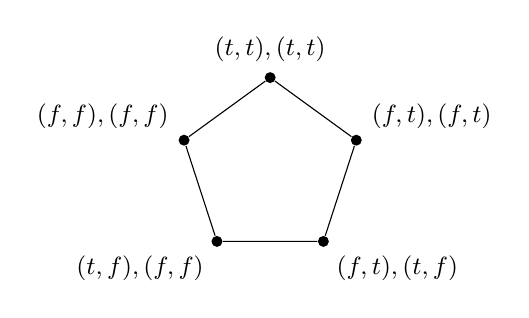
\begin{tikzpicture}[pt/.style={circle,fill,inner sep=1.4pt},
  every label/.style={font=\small}]
\node[pt,label={90:$(t,t),(t,t)$}]    (a) at (90:1.15) {};
\node[pt,label={18:$(f,t),(f,t)$}]    (b) at (18:1.15) {};
\node[pt,label={-54:$(f,t),(t,f)$}]   (c) at (-54:1.15) {};
\node[pt,label={-126:$(t,f),(f,f)$}]  (d) at (-126:1.15) {};
\node[pt,label={162:$(f,f),(f,f)$}]   (e) at (162:1.15) {};
\draw (a) -- (b) -- (c) -- (d) -- (e) -- (a);
\end{tikzpicture}
\caption{The five points of Theorem~\ref{thm:pentagon} over
$\mathrm{Bool}$, where $(a, b), (c, d)$ records $f(a) = b$ and
$g(c) = d$. Two points are joined when one pair of deterministic programs
produces both. The graph has no triangle, so the function with value
$\tfrac12$ on each point lies in $P(T)$. It has no three pairwise
non-adjacent points, so every randomized sequential program has total
weight at most $2$ on them.}
\label{fig:pentagon}
\end{figure}

\begin{theorem}[the pentagon\leanref{pente-not-mix}\leanref{pent-cycle}\leanref{pent-bounds}]
\label{thm:pentagon}
Let $X, Y, X', Y'$ have at least two elements each. There are five points
of the web of $T$ such that the function with value $\tfrac12$ on them and
$0$ elsewhere lies in $P(T)$ and not in the deterministic hull of $T$. For
$X = Y = X' = Y' = \mathrm{Bool}$, every randomized sequential program has
total weight at most $2$ on the five points, every element of $P(T)$ has
total weight at most $\tfrac52$ on them, and both bounds are attained.
\end{theorem}

\noindent
Over $\mathrm{Bool}$, write $(a, b)$ for the observation $f(a) = b$. The
five points are $((t,t),(t,t))$, $((t,f),(f,f))$, $((f,t),(t,f))$,
$((f,t),(f,t))$, and $((f,f),(f,f))$. They induce a cycle of length $5$ in the exclusivity graph
(Fig.~\ref{fig:pentagon}). The proof uses that this induced subgraph
has no triangle and no three pairwise non-adjacent vertices, which Lean checks by evaluation. It embeds the five points into larger types by
injections from $\mathrm{Bool}$. So no certain state gives the value $1$
to three of the five points. Hence $T$ has a gap: the function of the
theorem violates the counting law that bounds the total weight on the
five points by $2$.

The bounds $2$ and $\tfrac52$ are the independence number of the cycle
$C_5$ of length $5$, the largest number of pairwise non-adjacent vertices,
and its fractional relaxation. They are the noncontextual and the
exclusivity bounds of the KCBS scenario~\cite{cabello2014,klyachko2008}.

\subsection{Divergence and Total Programs}
\label{sec:second-total}

The function of Theorem~\ref{thm:pentagon} is partial: for some pairs of total functions it terminates with probability less
than $1$, for instance with probability $\tfrac12$ for $f$ the negation
and $g$ the identity on $\mathrm{Bool}$. At $T$ a
gap needs such partiality. Let $t \in P(T)$ terminate with probability $1$
on every pair of total functions. Constant arguments show that $t$ is a
conditional distribution of the inputs $(a, c)$ given the answers $(b, d)$. Termination with probability $1$ for all
total functions makes it a bipartite classical process without predefined causal
order~\cite{baumeler-wolf2016}. Every such process is a mixture of
processes in which one party acts first~\cite{baumeler-wolf2016}, and
these are randomized sequential programs. So $t$ lies in the deterministic hull of
$T$ by Theorem~\ref{thm:second-order}(ii). This argument is not
formalized. With three functional arguments,
we find a gap among the elements that terminate with probability $1$ on
every triple of total functions.

\begin{proposition}[a gap among total programs\leanref{gap-t3}]
\label{prop:t3}
Let $T_3 = ((\mathbf{2} \multimap \mathbf{2}) \otimes
(\mathbf{2} \multimap \mathbf{2}) \otimes
(\mathbf{2} \multimap \mathbf{2}))^{\perp}$. Some element of $P(T_3)$
terminates with probability $1$ on every triple of total functions and is
not in the deterministic hull of $T_3$.
\end{proposition}

\noindent
The element has value $1$ at one point of the web and $\tfrac12$ at
fourteen others. Since neither $\mathbf{2} \multimap \mathbf{2}$ nor its
tensor square has a gap, membership reduces to the $64$ triples of total
functions (proof of Theorem~\ref{thm:second-exact}). On each of them the
element has total weight exactly $1$. Five of its points with value
$\tfrac12$ form a cycle of length $5$ of exclusive pairs. So, as for
Theorem~\ref{thm:pentagon}, every mixture of certain states has total
weight at most $2$ on them, against $\tfrac52$. By the argument above,
the element is a tripartite classical process~\cite{baumeler-wolf2016}
that is not a mixture of deterministic ones. This identification is not
formalized.

% !TEX root = main.tex
\section{The Exact Condition}
\label{sec:exact}

This section describes the deterministic hull and the coherence space of $T$ as two
polytopes of one graph, and gives an exact condition for a gap at the dual
of a tensor of two formulas.

\subsection{$\STAB$ and $\QSTAB$}
\label{sec:exact-stab}

For a finite graph $G$ with vertex set $V$, a \emph{clique} is a set of
pairwise adjacent vertices and a \emph{stable set} a set of pairwise
non-adjacent vertices. The \emph{stable set polytope} $\STAB(G)$ is $\Mix$
of the indicators of the stable sets, and the \emph{clique-constrained
polytope} $\QSTAB(G)$ is the set of $x : V \to \mathbb{R}_{\ge 0}$ with
$\sum_{v \in C} x_v \le 1$ for every clique $C$~\cite{gls1988}. A stable
set meets every clique in at most one vertex, so
$\STAB(G) \subseteq \QSTAB(G)$. We prove that the two polytopes describe
the coherence space and the deterministic hull of $T$.

\begin{theorem}[graph polytopes\leanref{td-eq-qstab}\leanref{recipe-eq-stab}]
\label{thm:qstab}
Let $G$ be the exclusivity graph of $T$. Then $P(T) = \QSTAB(G)$, and the
deterministic hull of $T$ is $\STAB(G)$.
\end{theorem}

\noindent
Every element of $P(X \multimap Y)$ is a mixture of certain states
(Proposition~\ref{prop:first-order}). Every certain state lies below
the indicator of the graph of a total function. So $P(T)$ is cut out by
the products of two such indicators. Their supports are the maximal
cliques of $G$, so $P(T) = \QSTAB(G)$. An element of $\QSTAB(G)$ with values in $\{0,1\}$
is the indicator of a stable set, so the deterministic hull is $\STAB(G)$.

So $T$ has a gap iff $\STAB(G) \ne \QSTAB(G)$. A graph is \emph{perfect}
if every induced subgraph has chromatic number equal to its largest
clique size. Then $\STAB(G) = \QSTAB(G)$ iff $G$ is
perfect~\cite{lovasz1972,chvatal1975}. The cycle of length $5$ of
Theorem~\ref{thm:pentagon} is an induced subgraph of $G$ that is not
perfect.

\subsection{The Clique Property and Perfection}
\label{sec:exact-perfect}

A formula $X$ has the \emph{clique property} if $P(X)$ is the set of
mixtures of the indicators of the cliques of its coherence graph $G_X$.
Data types, their negations, and the formulas $\mathbf{n} \multimap
\mathbf{m}$ (Proposition~\ref{prop:first-order}) have it. So does every
formula built from data types with $\mathbin{\&}$ and $\oplus$, since
$P(A \mathbin{\&} B)$ is the product of $P(A)$ and $P(B)$ and
$P(A \oplus B)$ is the convex hull of the copies of $P(A)$ and $P(B)$ on
the two parts of the web~\cite{danos-ehrhard2011}. Lean checks this for the
formulas built from the data type $\mathbf{1}$ with $\mathbin{\&}$ and
$\oplus$\leanref{recipe-code}. Their coherence graphs are the
\emph{cographs}, the graphs with no induced path on four
vertices~\cite{corneil1981}, with $\mathbin{\&}$ as join, which adds all
edges between the two parts, and $\oplus$ as disjoint union.

An \emph{induced $4$-cycle} of a formula $X$ is a quadruple of points
$a, b, c, d$ with $a \coh b \coh c \coh d \coh a$ and with $a, c$ and
$b, d$ incoherent. The \emph{strong product} $G \boxtimes H$ of two
graphs has the pairs of vertices as vertices, and two distinct pairs are
adjacent iff each coordinate is equal or adjacent. By
Definition~\ref{def:mall}(iv), the coherence graph of $X \otimes Y$ is
$G_X \boxtimes G_Y$. We prove the following exact condition.

\begin{theorem}[second order\leanref{closure}\leanref{recipe-core}\leanref{second-iff}]
\label{thm:second-exact}
Let $X$ and $Y$ have the clique property.
(i) $X \otimes Y$ has no gap. Moreover, $(X \otimes Y)^{\perp}$ has no gap
iff
$G_X \boxtimes G_Y$ is perfect.
(ii) If $G_X$ and $G_Y$ are cographs, then $(X \otimes Y)^{\perp}$ has no
gap iff $G_X$ or $G_Y$ has no induced $4$-cycle.
\end{theorem}

\noindent
If neither $X$ nor $Y$ has a gap, then neither do $X \otimes Y$,
$X \mathbin{\&} Y$, and $X \oplus Y$. Moreover, $P((X \otimes Y)^{\perp})$ is
cut out by the products of the certain states of $X$ and of $Y$. The Lean proof shows a bipolar theorem for downward-closed sets of
$\{0,1\}$-valued functions by hyperplane separation, as for the
completeness theorem of Section~\ref{sec:calculi}. With the
clique property these products are the indicators of the products
$K \times L$ of cliques, which are the maximal cliques of
$F = G_X \boxtimes G_Y$. So $P((X \otimes Y)^{\perp}) = \QSTAB(F)$, and its certain states are the
indicators of the stable sets of $F$. The deterministic hull is therefore $\STAB(F)$, which equals $\QSTAB(F)$ iff $F$ is
perfect. In (ii), the gap when both graphs
have an induced $4$-cycle follows from Theorem~\ref{thm:c4}, which holds for all
formulas. The closure statements, the description of
$P((X \otimes Y)^{\perp})$ as the orthogonal of the products of certain
states, and (ii) for $X$ and $Y$ built from $\mathbf{1}$ with
$\mathbin{\&}$ and $\oplus$ are formalized. The description as
$\QSTAB(F)$ is formalized at $T$ (Theorem~\ref{thm:qstab}), and the
equivalence with perfection in (i) is cited.

For $X = \mathbf{n} \multimap \mathbf{m}$ the coherence graph is complete
multipartite, with the inputs as the $n$ classes of $m$ points each and
two points adjacent iff they lie in different classes. It has an induced
$4$-cycle iff $n, m \ge 2$: two points in each of two classes form one,
for $n = 1$ the graph has no edges, and for $m = 1$ it is complete. So $T$ has a gap iff each of $X, Y, X', Y'$
has at least two elements, and the core has no gap\leanref{recipe-core}.
The gap when all four have at least two elements follows from Theorem~\ref{thm:pentagon}. The absence of a gap otherwise uses (ii) for
formulas not built from $\mathbf{1}$, through the transfer below, which is
not formalized.

\subsection{Four-Cycles: a Direct Proof}
\label{sec:exact-direct}

We prove the direction of (ii) without a gap by an explicit
decomposition, without perfect graph theory. If neither side of
$A \mathbin{\&} B$ is a clique, an incoherent pair in $A$ and one in $B$
form an induced $4$-cycle. So a formula built from $\mathbf{1}$ with
$\mathbin{\&}$ and $\oplus$ that has no induced $4$-cycle is isomorphic,
by a bijection of the webs that preserves coherence in both directions, to
one built from $\mathbf{1}$ with $\oplus$ and
$A \mapsto A \mathbin{\&} \mathbf{1}$\leanref{tree-of-noc4}. Its points
are the nodes of a rooted forest, and two points cohere iff one lies on the
path from a root to the other. So $G_X$ is the comparability graph of the
forest~\cite{wolk1962,golumbic1978}. For $v : |Y| \to \mathbb{R}_{\ge 0}$
let $\omega(v)$ be the largest total weight of a clique of $G_Y$. Then
$z$ lies in $P((X \otimes Y)^{\perp})$ iff
$\omega(\sum_{x \in \pi} z(x, \cdot)) \le 1$ for every path $\pi$ from a
root\leanref{mem-p-iff}. Every such $z$ is a mixture of
$\{0,1\}$-valued functions whose sums along the paths are indicators of
stable sets of $G_Y$\leanref{decompose}. The proof is an induction on the
forest, whose step at a root is an induction on $Y$. At $\oplus$ the two
components are decomposed separately. At $\mathbin{\&}$ a stable set lies
in one component, and is drawn there with probability given by $\omega$,
after a split of the weights below the root that keeps $\omega$ within its
level along every path\leanref{absorb}.

Lean checks (ii) in both directions for $X$ and $Y$ built from
$\mathbf{1}$ with $\mathbin{\&}$ and $\oplus$\leanref{second-iff}. For the
other formulas in (ii) with nonempty webs, the clique property makes a
coherence-preserving bijection onto such a formula preserve the coherence spaces. This transfer is not formalized. With the cited part of (i), the proof shows that the strong product of a
forest comparability graph and a cograph is perfect. This consequence is
not formalized. This extends the theorem that the strong product of two forest
comparability graphs, the graphs with no induced path on four vertices
and no induced $4$-cycle, is perfect~\cite{ravindra1978}. We did not find the extension in the literature.

\subsection{Beyond Second Order}
\label{sec:exact-beyond}

An occurrence of a formula $D$ in a formula $A$ is \emph{positive} if it
lies under an even number of negations and \emph{negative} otherwise, the
derived connectives $\parr$, $\oplus$, and $\multimap$ being unfolded. So
the left argument of $\multimap$ is a negative position. Beyond second
order, we find a gap even when no negatively occurring tensor has an
induced $4$-cycle in both factors.

\begin{proposition}[a gap without four-cycles\leanref{gap-f3}]
\label{prop:f3}
The formula $(\mathbf{2} \mathbin{\&} \mathbf{1}) \multimap
((\mathbf{2} \multimap \mathbf{2}) \otimes (\mathbf{2} \multimap
\mathbf{2}))$ has a gap. Every tensor occurring negatively in it has a
factor with at most three points, so none has an induced $4$-cycle in
both factors.
\end{proposition}

\noindent
The formula is $((\mathbf{2} \mathbin{\&} \mathbf{1}) \otimes T)^{\perp}$.
An element outside the deterministic hull has value $\tfrac12$ at five points of the
web. Its membership in the coherence space uses the bounds of Theorem~\ref{thm:mall} at three incoherent pairs and
at one point of $T$. The five points form an induced cycle of length $5$ in the
coherence graph, so by Theorem~\ref{thm:mall} every certain state is $1$
at no more than two of them. So every mixture has total weight at most $2$
there, against $\tfrac52$. The second statement of the proposition is
checked by inspection of the formula.

% !TEX root = main.tex
\section{Other Formulas}
\label{sec:other}

A gap transfers along a kind of embedding of webs. This section uses it
to carry the gap of Theorem~\ref{thm:pentagon} to every formula with a
negative occurrence of a suitable tensor.

\subsection{Coordinate Retracts}
\label{sec:other-retract}

\begin{definition}[coordinate retract\leanref{retract}]
\label{def:retract}
For given formulas $D$ and $A$, the \emph{coordinate retracts} of $D$
into $A$ are the injective maps $j : |D| \to |A|$ such that the
pushforward $j_{*}$, defined by $(j_{*}x)(j(d)) = x_d$ and value $0$
outside the image of $j$, maps $P(D)$ into $P(A)$, and the pullback
$z \mapsto z \circ j$ maps $P(A)$ into $P(D)$. We say that $D$ is a
coordinate retract of $A$ if such a map exists.
\end{definition}

\noindent
The pullback of $j_{*}x$ is $x$, and this allows us to prove that gaps
transfer along coordinate retracts.

\begin{theorem}[transfer\leanref{retract-gap}\leanref{retract-ops}]
\label{thm:retract}
(i) If $D$ is a coordinate retract of $A$ and $D$ has a gap, then $A$ has
a gap.
(ii) Coordinate retracts compose. If $D$ is a coordinate retract of $A$,
then $D^{\perp}$ is a coordinate retract of $A^{\perp}$. The formula $D$
is a coordinate retract of $D \mathbin{\&} B$, of $B \mathbin{\&} D$,
and, if the web of $B$ is nonempty, of $D \otimes B$ and of $B \otimes D$.
\end{theorem}

\noindent
For (i), take $x \in P(D)$ outside the deterministic hull of $D$. If $j_{*}x$ were a
mixture of certain states of $A$, pulling the mixture back along $j$
would write $x = (j_{*}x) \circ j$ as a mixture of certain states of $D$.
For negation, the pairing satisfies
$\langle j_{*}u, z \rangle = \langle u, z \circ j \rangle$, which exchanges
the two conditions of Definition~\ref{def:retract}. For $D \otimes B$,
the map is $j(d) = (d, b)$ for a point $b$ of $B$, so
$j_{*}x = x \otimes \delta_b$, where $\delta_b$ is the indicator of $b$. The pullback condition uses that every element of $P(B)$ is at most
$1$ at $b$ (Theorem~\ref{thm:mall}).

\subsection{Negative Occurrences and Four-Cycles}
\label{sec:other-occ}

With positive and negative occurrences as defined in
Section~\ref{sec:exact-beyond}, we prove the following.

\begin{theorem}[the gap at other formulas\leanref{gap-of-occ}]
\label{thm:occ-gap}
Let $n, m, n', m' \ge 2$, and let $A$ be a formula all of whose data types
are nonempty. If $(\mathbf{n} \multimap \mathbf{m}) \otimes
(\mathbf{n'} \multimap \mathbf{m'})$ occurs negatively in $A$, then $A$
has a gap.
\end{theorem}

\noindent
A positive occurrence of $D$ gives a coordinate retract of $D$ into $A$,
and a negative one a coordinate retract of $D^{\perp}$, by
Theorem~\ref{thm:retract}(ii) and induction on $A$, using that $D$ is a
coordinate retract of $D^{\perp\perp}$. Theorem~\ref{thm:retract}(i) and
Theorem~\ref{thm:pentagon} then give the claim. Examples are $T$ itself,
the type $((\mathbf{n} \multimap \mathbf{m}) \otimes (\mathbf{n'}
\multimap \mathbf{m'})) \multimap B$ of a program that receives two
functions and returns a value of type $B$, for every $B$ with nonempty
data types (Lean checks the instance $B = \mathbf{2}$). A positive occurrence of the core
does not suffice: the core itself has no gap
(Theorem~\ref{thm:second-exact}(i)).

The occurrence condition of Theorem~\ref{thm:occ-gap} refers to one
syntactic subformula. We also prove a version that depends only on the
coherence graphs of the factors.

\begin{theorem}[four-cycles\leanref{retract-tens}\leanref{c4-retract}\leanref{gap-of-c4}]
\label{thm:c4}
If $X$ and $Y$ both have an induced $4$-cycle, then
$(X \otimes Y)^{\perp}$ has a gap, and so does every formula over
nonempty data types in which $X \otimes Y$ occurs negatively.
\end{theorem}

\noindent
The four points of an induced $4$-cycle of $X$ form a coordinate retract of
$\mathbf{2} \multimap \mathbf{2}$ into $X$, with input $0$ sent to $a$ and
$c$ and input $1$ to $b$ and $d$. The pushforward lands in $P(X)$ because
the indicators of the coherent pairs of the cycle lie in $P(X)$ (Theorem~\ref{thm:mall}). The pullback lands in
$P(\mathbf{2} \multimap \mathbf{2})$ because the incoherent pairs have
total weight at most $1$ (Theorem~\ref{thm:mall}). Coordinate retracts
pass through $\otimes$, so Theorems~\ref{thm:pentagon}
and~\ref{thm:retract} give the claim. The coherence graph of
$\mathbf{n} \multimap \mathbf{m}$ has an induced $4$-cycle iff
$n, m \ge 2$, so Theorem~\ref{thm:occ-gap} is the case
$X = \mathbf{n} \multimap \mathbf{m}$ and
$Y = \mathbf{n'} \multimap \mathbf{m'}$. The curried type $(\mathbf{2} \multimap
\mathbf{2}) \multimap ((\mathbf{2} \multimap \mathbf{2}) \multimap
\mathbf{2})$, which Theorem~\ref{thm:occ-gap} does not cover, is an
instance\leanref{gap-curried}.

% !TEX root = main.tex
\section{Local Certainty and Duality}
\label{sec:duality}

The deterministic hull mixes states that are certain on all events at once. A
weaker requirement is certainty within each of a family of contexts. This section places the PCS between the deterministic hull
and the resulting local relaxation. It ends with a quantum event logic,
which has no certain states.

\subsection{The Local Relaxation}
\label{sec:duality-local}

\begin{definition}[local relaxation~\cite{acin2015}\leanref{local-calc}]
\label{def:local}
For a given finite set $E$ of events and a family $\mathcal{C}$ of
subsets of $E$, the \emph{contexts}, the \emph{local relaxation} is the set
of $x : E \to \mathbb{R}_{\ge 0}$ such that $\sum_{e \in C} x_e \le 1$
for every context $C$. The \emph{deterministic hull} is $\Mix$ of the
elements of the local relaxation with values in $\{0,1\}$. The
\emph{normalized} local relaxation and deterministic hull are the sets defined in the
same way with $=$ in place of $\le$.
\end{definition}

\noindent
The local relaxation contains its
$\{0,1\}$-valued elements and is closed under mixtures, so
Definition~\ref{def:gap} applies to it, with the deterministic hull as
$\Mix$ of its certain states. The normalized local relaxation and deterministic hull are
the general probabilistic models and the classical models of a family of
contexts~\cite{acin2015}.

For a formula $A$, take as contexts the supports of the certain states of
$A^{\perp}$. The pairing with a $\{0,1\}$-valued function is the sum over
its support, so the local relaxation of $A$ is the orthogonal of the certain
states of $A^{\perp}$\leanref{loc-linear}. We write $\loc(A)$ for it,
and we prove that it bounds the PCS from above.

\begin{theorem}[local certainty\leanref{loc-linear}\leanref{recipe-core}\leanref{recipe-formula}]
\label{thm:loc-linear}
For every formula $A$, the deterministic hull of $A$ is contained in $P(A)$, which is contained in $\loc(A)$. Moreover, $P(A) = \loc(A)$ iff $A^{\perp}$
has no gap.
At $T$ the second inclusion is an equality, and if $X, Y, X', Y'$ have at
least two elements each, the first is strict.
\end{theorem}

\noindent
An orthogonal does not change when a set is replaced by its mixtures, so
$\loc(A)$ is the orthogonal of the deterministic hull of $A^{\perp}$. By
Definition~\ref{def:mall}(iii), $P(A)$ is the orthogonal of $P(A^{\perp})$. The deterministic hull of $A^{\perp}$ is contained
in $P(A^{\perp})$, which gives $P(A) \subseteq \loc(A)$. The deterministic hull and
the PCS of every formula are equal to their biorthogonals, the
deterministic hull by the bipolar theorem in the proof of
Theorem~\ref{thm:second-exact}, which gives the equivalence. At $T$ the dual is the core, which has no gap
(Theorem~\ref{thm:second-exact}(i)), and the first inclusion is strict by
Theorem~\ref{thm:pentagon}.

\subsection{A Clique Outside the PCS}
\label{sec:duality-shannon}

The converse of the last statement of Theorem~\ref{thm:mall} fails: some
cliques of the coherence graph are not certain states. Let
$X = Y = X' = Y' = \mathrm{Bool}$. On the five points of
Theorem~\ref{thm:pentagon}, two distinct points cohere in $T$ iff they are
not exclusive. Order them as $c_0, \dots, c_4$ along the cycle of length
$5$ of the exclusivity graph. The coherence graph on them is the
complement of this cycle, again a cycle of length $5$. Two distinct points
of $T \otimes T$ are incoherent iff they are incoherent in one component,
so a clique of $(T \otimes T)^{\perp}$ contained in
$\{c_0, \dots, c_4\}^2$ is a stable set of the strong product of two
cycles of length $5$. The set $\{(c_i, c_{2i}) \mid i \in \mathbb{Z}/5\}$
is such a stable set, of size $5$, Shannon's stable
set~\cite{lovasz1979}. We show that it gives a clique outside the
PCS.

\begin{theorem}[a clique outside the PCS\leanref{shannon-clique}\leanref{shannon-not-mem}\leanref{tensorgap-bool}]
\label{thm:shannon}
Shannon's set is a clique of the coherence graph of $(T \otimes T)^{\perp}$,
and its indicator does not lie in $P((T \otimes T)^{\perp})$.
\end{theorem}

\noindent
The function $z$ of Theorem~\ref{thm:pentagon}, with value $\tfrac12$ on
the five points, lies in $P(T)$, so $z \otimes z$ lies in $P(T \otimes T)$.
Its pairing with the indicator of Shannon's set is
$5 \cdot \tfrac14 = \tfrac54 > 1$.

The indicator of every clique of $A$ lies in $\loc(A)$. The certain
states of $A^{\perp}$ are cliques of $A^{\perp}$ (Theorem~\ref{thm:mall}). A clique of $A$ and a
clique of $A^{\perp}$ share at most one point,
since two distinct points cannot cohere in both. This allows us to prove
that Shannon's set also separates the PCS from the local
relaxation.

\begin{corollary}[the second inclusion\leanref{loc-linear}]
\label{cor:tt}
At $(T \otimes T)^{\perp}$, the PCS is strictly contained in
the local relaxation.
\end{corollary}

\noindent
The first inclusion is strict there too, by Theorem~\ref{thm:c4}: the
points $((t,t),(t,t))$, $((t,t),(t,f))$, $((f,t),(t,t))$, $((f,t),(t,f))$
form an induced $4$-cycle of $T$\leanref{tt-gap}.
We did not find the placement of the PCS between the
deterministic hull and the local relaxation
(Theorem~\ref{thm:loc-linear}) in the literature.

\subsection{Negation, Tightness, and the Tensor}
\label{sec:duality-tight}

Two sets $U$ and $V$ of weight vectors on one web form a \emph{tight
pair} if each is the orthogonal of the other, $U = V^{\perp}$ and
$V = U^{\perp}$~\cite{hyland-schalk2003}. A PCS and its
orthogonal form a tight pair. The question is when the deterministic hulls of a formula and of its negation form a tight
pair, and we prove the following answer, whose part (i) extends the
antiblocking duality below.

\begin{theorem}[duality\leanref{orth-recipe}\leanref{tight}]
\label{thm:duality}
Let $A$ be a formula.
(i) The orthogonal of the deterministic hull of $A$ is $\loc(A^{\perp})$, and the
orthogonal of $\loc(A)$ is the deterministic hull of $A^{\perp}$.
(ii) The deterministic hulls of $A$ and of $A^{\perp}$ form a tight pair iff the
deterministic hull of $A$ is $\loc(A)$, iff neither $A$ nor $A^{\perp}$ has a gap.
(iii) If $X, Y, X', Y'$ have at least two elements each, the deterministic hulls of
the core $K$ and of $T$ do not form a tight pair.
\end{theorem}

\noindent
Part (i) combines the biorthogonal closure of the deterministic hull with the fact
that an orthogonal does not change when a set is replaced by its
mixtures. Each of the two equations of a tight pair of deterministic hulls implies the
other, since the deterministic hull is equal to its biorthogonal. Part (ii) follows
with Theorem~\ref{thm:loc-linear}, and (iii)
with Theorem~\ref{thm:second-exact}(i) and the gap at $T$
(Theorem~\ref{thm:pentagon}).

When the certain states of $A$ and of $A^{\perp}$ are the cliques of their
coherence graphs, (i) is the antiblocking identity between the stable set
polytope of a graph and the clique-constrained polytope of its
complement, which joins two distinct vertices iff the graph does
not~\cite{fulkerson1971,knuth1994}. In that case tightness holds iff the
coherence graph is perfect~\cite{lovasz1972,chvatal1975}. For a coherence space $E$ in the sense of Girard, let $p(E)$ be the set of $x \ge 0$ with total
weight at most $1$ on every clique of $E^{\perp}$. Then
$p(E^{\perp}) = p(E)^{\perp}$ when $E$ is generated from $\mathbf{1}$ by
$\perp$ and $\mathbin{\&}$, so that its coherence graph is a cograph, and
not when its coherence graph has an induced cycle of length
$5$~\cite{ehrhard-td2}. A family of finite sets and its orthogonal family
have dual norm balls iff they are the cliques and the stable sets of a
perfect graph~\cite{bfp2026}. These results concern the cliques of a coherence graph.
Theorem~\ref{thm:duality} concerns its certain states, which can be fewer
than the cliques (Theorem~\ref{thm:shannon}). To our knowledge, part (ii), the equivalence of tightness with the
absence of a gap at $A$ and at $A^{\perp}$, does not appear in the
literature.

We show that tightness holds at first order and fails at a tensor of
first-order types.

\begin{corollary}[tightness and the tensor\leanref{tight-tensor}]
\label{cor:tensor}
For all $n$ and $m$, the local relaxation of $\mathbf{n} \multimap
\mathbf{m}$ is $P(\mathbf{n} \multimap \mathbf{m})$, so the deterministic hulls of
$\mathbf{n} \multimap \mathbf{m}$ and of its negation form a tight pair.
For $n, m, n', m' \ge 2$, the deterministic hulls of $(\mathbf{n} \multimap
\mathbf{m}) \otimes (\mathbf{n'} \multimap \mathbf{m'})$ and of its
negation do not.
\end{corollary}

\noindent
The indicator of a row $\{a\} \times \{1, \dots, m\}$ is a certain state
of the negation of $\mathbf{n} \multimap \mathbf{m}$. These indicators cut
out the row-substochastic matrices, which form
$P(\mathbf{n} \multimap \mathbf{m})$. With
Proposition~\ref{prop:first-order} the deterministic hull is the local relaxation. The
second statement is Theorem~\ref{thm:duality} with the gap of
Theorem~\ref{thm:pentagon}. So tightness at $A$ and at $B$ does not
imply tightness at $A \otimes B$, although $P(A \otimes B)$ is determined
by $P(A)$ and $P(B)$ (Definition~\ref{def:mall}(iii)).

\subsection{Bell's Theorem at the Core}
\label{sec:duality-bell}

Let $X = Y = X' = Y' = \mathbf{2}$. A point $((x, a), (y, b))$ of the web
of the core $K$ is the event that two parties with inputs $x$ and $y$ give
outputs $a$ and $b$. Two events are \emph{locally orthogonal} if some
party has equal inputs and different outputs. For distinct events this is the negation of exclusivity
(Section~\ref{sec:second-pentagon}). An element of $P(K)$ is \emph{normalized} if it has total
weight $1$ for each pair of inputs. The second statement of the following
form of Bell's theorem is known~\cite{bell1964,chsh1969,popescu-rohrlich1994},
the first restates Theorem~\ref{thm:qstab}, and we formalize both.

\begin{theorem}[Bell at the core~\cite{bell1964,popescu-rohrlich1994}\leanref{bell}]
\label{thm:bell}
Every certain state of $T$ is the indicator of a set of pairwise locally
orthogonal events. The Popescu--Rohrlich box~\cite{popescu-rohrlich1994},
with value $\tfrac12$ on the
events with $a + b \equiv xy \pmod 2$ and $0$ elsewhere, lies in
$\loc(K)$ and not in $P(K)$.
\end{theorem}

\noindent
Two events that are not locally orthogonal are both produced by one
deterministic product strategy, a pair of deterministic programs, one for
each party, which lies in $P(K)$ and has pairing $2$ with their
indicator. No three events in the support of the box are pairwise
locally orthogonal, so the box has total weight at most $1$ on the support
of every certain state of $T$, and lies in $\loc(K)$. By
Theorem~\ref{thm:second-exact}, $P(K)$ is the deterministic hull of $K$. Every
certain state of $K$ lies below a deterministic product strategy, which
has total weight at most $3$ on the eight events with $a + b \equiv xy$,
the CHSH inequality~\cite{chsh1969}. The box has total weight $4$ there.
By Theorem~\ref{thm:loc-linear}, $P(K) \ne \loc(K)$ iff $T$ has a gap.

The normalized elements of $P(K)$ are the Bell-local behaviours, i.e. the
mixtures of deterministic product strategies that always terminate. A set
of pairwise locally orthogonal events meets each clique of $K$ in at most
one event, so $\loc(K)$ is the set of functions with total weight at most
$1$ on every such set. Its normalized elements are the no-signalling
behaviours~\cite{fritz-lo2013}. These two identifications are not
formalized.

% !TEX root = main.tex
\subsection{Quantum Event Logic}
\label{sec:quantum}

In quantum logic, the events are the closed subspaces of a Hilbert
space~\cite{birkhoff-vonneumann1936}. A context is an orthogonal
basis, a maximal set of pairwise orthogonal rays. We take as events the
$18$ rays of Cabello's set in $\mathbb{R}^4$, spanned by vectors with
coordinates in $\{0, \pm 1\}$, and as contexts its $9$ orthogonal bases,
each ray lying in exactly two of them~\cite{cabello1996}\leanref{cabello-set}\leanref{basis-orth}.
We write $1\bar{1}00$ for the ray spanned by $(1, -1, 0, 0)$. A
\emph{state} is an element of the normalized local relaxation of
Definition~\ref{def:local}. For a unit vector $\psi$, the \emph{Born rule}
gives the ray spanned by $v$ the value $x_v = (\psi \cdot v)^2 / (v \cdot v)$. This is a state\leanref{born-state}\leanref{parseval}. The mixtures of these states are
the \emph{quantum states}.

The construction of Section~\ref{sec:calculi} gives the empty deterministic hull
here: no state has values in
$\{0,1\}$~\cite{kochen-specker1967,cabello1996}, so the normalized deterministic
hull is empty. We formalize this known
fact\leanref{no-ks}\leanref{no-certain-state}. We also prove that the
normalized local relaxation contains states that are not mixtures of
Born-rule assignments of these rays.

\begin{theorem}[local certainty in quantum logic\leanref{loc-quantum}]
\label{thm:loc-quantum}
On Cabello's set, the function $h$ with value $\tfrac12$ on the nine rays
$\bar{1}111$, $0001$, $0010$, $0100$, $1\bar{1}\bar{1}1$,
$1\bar{1}1\bar{1}$, $11\bar{1}1$, $111\bar{1}$, $1111$ and $0$ elsewhere is
a state and is not a mixture of Born-rule assignments.
\end{theorem}

\noindent
Every basis contains exactly two of the nine rays, so $h$ is a state. The
ray $0001$ lies in the plane of the orthogonal rays $1001$ and
$100\bar{1}$, so every Born-rule assignment satisfies
$x_{0001} \le x_{1001} + x_{100\bar{1}}$, the difference being
$\psi_1^2$. The function $h$ violates this law, with values $\tfrac12$,
$0$, and $0$. No basis contains $0001$ and either of the other two rays,
while each condition of the local relaxation involves a single basis.

In Theorem~\ref{thm:loc-quantum}, each ray $v$ is represented by the
projection onto $v$ in $\mathbb{R}^4$. A state $x$ has a \emph{quantum
model} if some Hilbert space has a projection $P_v$ for each ray $v$,
summing to the identity on each basis, and a positive operator
$\rho$ of trace $1$ with $x_v = \mathrm{tr}(\rho P_v)$ for every ray $v$.
Whether every state on Cabello's set has a quantum model was left
open~\cite{acin2015}. The state $h$ has none in finite dimension. It is
the only state that vanishes outside its nine rays, so it is an extreme point of the set of states. This step is not
formalized. An extreme state with a value outside
$\{0,1\}$ has no quantum model~\cite{sujan-kunjwal2025}. On all rays of $\mathbb{R}^d$
with $d \ge 3$, every state is a quantum state~\cite{gleason1957}.

% !TEX root = main.tex
\section{Related Work}
\label{sec:related}

\textbf{Probabilistic semantics.}
In quasi-Borel spaces, a
model of higher-order probability, every distribution is the image of a
distribution on the real line under a map into the
space~\cite{heunen2017qbs}. The elements of a probabilistic coherence
space are not given in this form.

\textbf{Generalized probabilism.}
The construction of Section~\ref{sec:calculi} is generalized
probabilism~\cite{paris2001,williams2012}. The laws valid on all truth
assignments to a set of events are Boole's conditions of possible
experience~\cite{pitowsky1994}. Other
derivations obtain the sum and product rules of probability from
properties of a lattice of events~\cite{cox1946,vanhorn2003,knuth-skilling2012}.
In these approaches the events are formulas or lattice elements. For a formula, the events are the points of its web, which carry no
connectives.

\textbf{Probabilistic theories and contextuality.}
Generalized probabilistic theories describe a system by its states and
its effects, the outcomes of measurements~\cite{barrett2007,plavala2023},
and under the no-restriction hypothesis every map from states to $[0,1]$
that respects mixtures is an effect~\cite{janotta-lal2013}. Contextuality has
combinatorial formulations by exclusivity graphs~\cite{cabello2014}, by
hypergraphs of contexts~\cite{acin2015}, and by
sheaves~\cite{abramsky-brandenburger2011}. Its noncontextual models form
correlation polytopes~\cite{pitowsky1991}, and it also occurs in other
domains~\cite{abramsky2013}. In these formulations the scenario is given
by its measurements and outcomes. Here, we work with webs of a type, with
exclusivity defined by coherence.

\textbf{Causal processes.}
Probabilistic coherence spaces model the deep-inference logic BV, which
adds a noncommutative connective for sequential
composition~\cite{blute-panangaden-slavnov2012}. Higher-order causal
theories, built from categories of processes compatible with a causal
order~\cite{kissinger-uijlen2019}, also model BV. Over matrices of nonnegative numbers they give this model of probabilistic coherence spaces
restricted to normalized maps~\cite{simmons-kissinger2022}.

% !TEX root = main.tex
\section{Conclusion}
\label{sec:conclusion}

At first order the PCS of a type is the set of mixtures of
deterministic programs. At second order it also contains behaviours that
no randomized sequential program has, and induced four-cycles decide when
this happens. So a law of sequential programs, such as the KCBS
inequality, need not hold in the model. By duality the gap is equivalent
to Bell's theorem at the dual type, and the tensor does not preserve
tightness of the deterministic hulls.

These results bear on three uses of the model. First, arguments that
replace a randomized program by a distribution over deterministic ones, as
in Yao's minimax principle~\cite{yao1977}, are valid in the model exactly
at the types without a gap, such as the first-order types, and not at $T$ over $\mathrm{Bool}$. Second, a bound proved over a PCS holds for every program
of its type, and the deterministic hull shows when it is tight. On the
five points of the pentagon, the PCS allows total weight
$\tfrac52$, while every sequential program has at most $2$. Third, if the
environments of a categorical framework for composable
security~\cite{broadbent-karvonen2022} are interpreted in
PCS, they include non-sequential ones, so security proved against them
is stronger than security against programs.

Open questions include other models of probabilistic programs, an exact
condition beyond second order, where the coherence graphs are not
cographs, and the exponential types. The theta body of a graph lies
between its stable set and clique-constrained polytopes and gives the
quantum bounds of a contextuality scenario~\cite{cabello2014}, so it may
describe programs with quantum resources. A comparison with categories of
processes compatible with a causal order~\cite{kissinger-uijlen2019} is
also open.


\section*{Disclosure of Generative AI Use}
A generative artificial intelligence (AI) assistant (Claude, Anthropic) was used to draft and edit
the text, to search the literature, and to develop parts of the Lean
formalization. The authors checked every statement, proof, citation and
Lean result, and take full responsibility for the content.

\section*{Data Availability Statement}
The Lean~4 development that mechanizes every result marked with a
superscript number such as \textsuperscript{\textsf{\scriptsize L1}} is
available as an anonymized archive at
\url{https://doi.org/10.5281/zenodo.23351908}. It builds with
\textsf{mathlib}, contains no \texttt{sorry}, and uses only the axioms
\texttt{propext}, \texttt{Classical.choice}, and \texttt{Quot.sound}. The
archive also contains a document that lists the numbered Lean statements.
The development will be submitted for artifact evaluation.

\bibliographystyle{splncs04}
\bibliography{refs}

\end{document}
